\subsection{Aggiunta Pannello alla Dashboard}\label{AddPanel}

Una volta effetuato l'accesso a \textit{Grafana} è necessario per prima cosa aggiungere alla propria Dashboard il pannello \textit{G\&B}. Gli utenti con esperienza nell'uso della piattaforma \textit{Grafana} non dovrebbero aver problemi in tal senso, ciò nonostante forniamo una descrione di questa operazione per chi ne avesse bisogno.\\

\begin{figure}[H]
	\begin{center}
		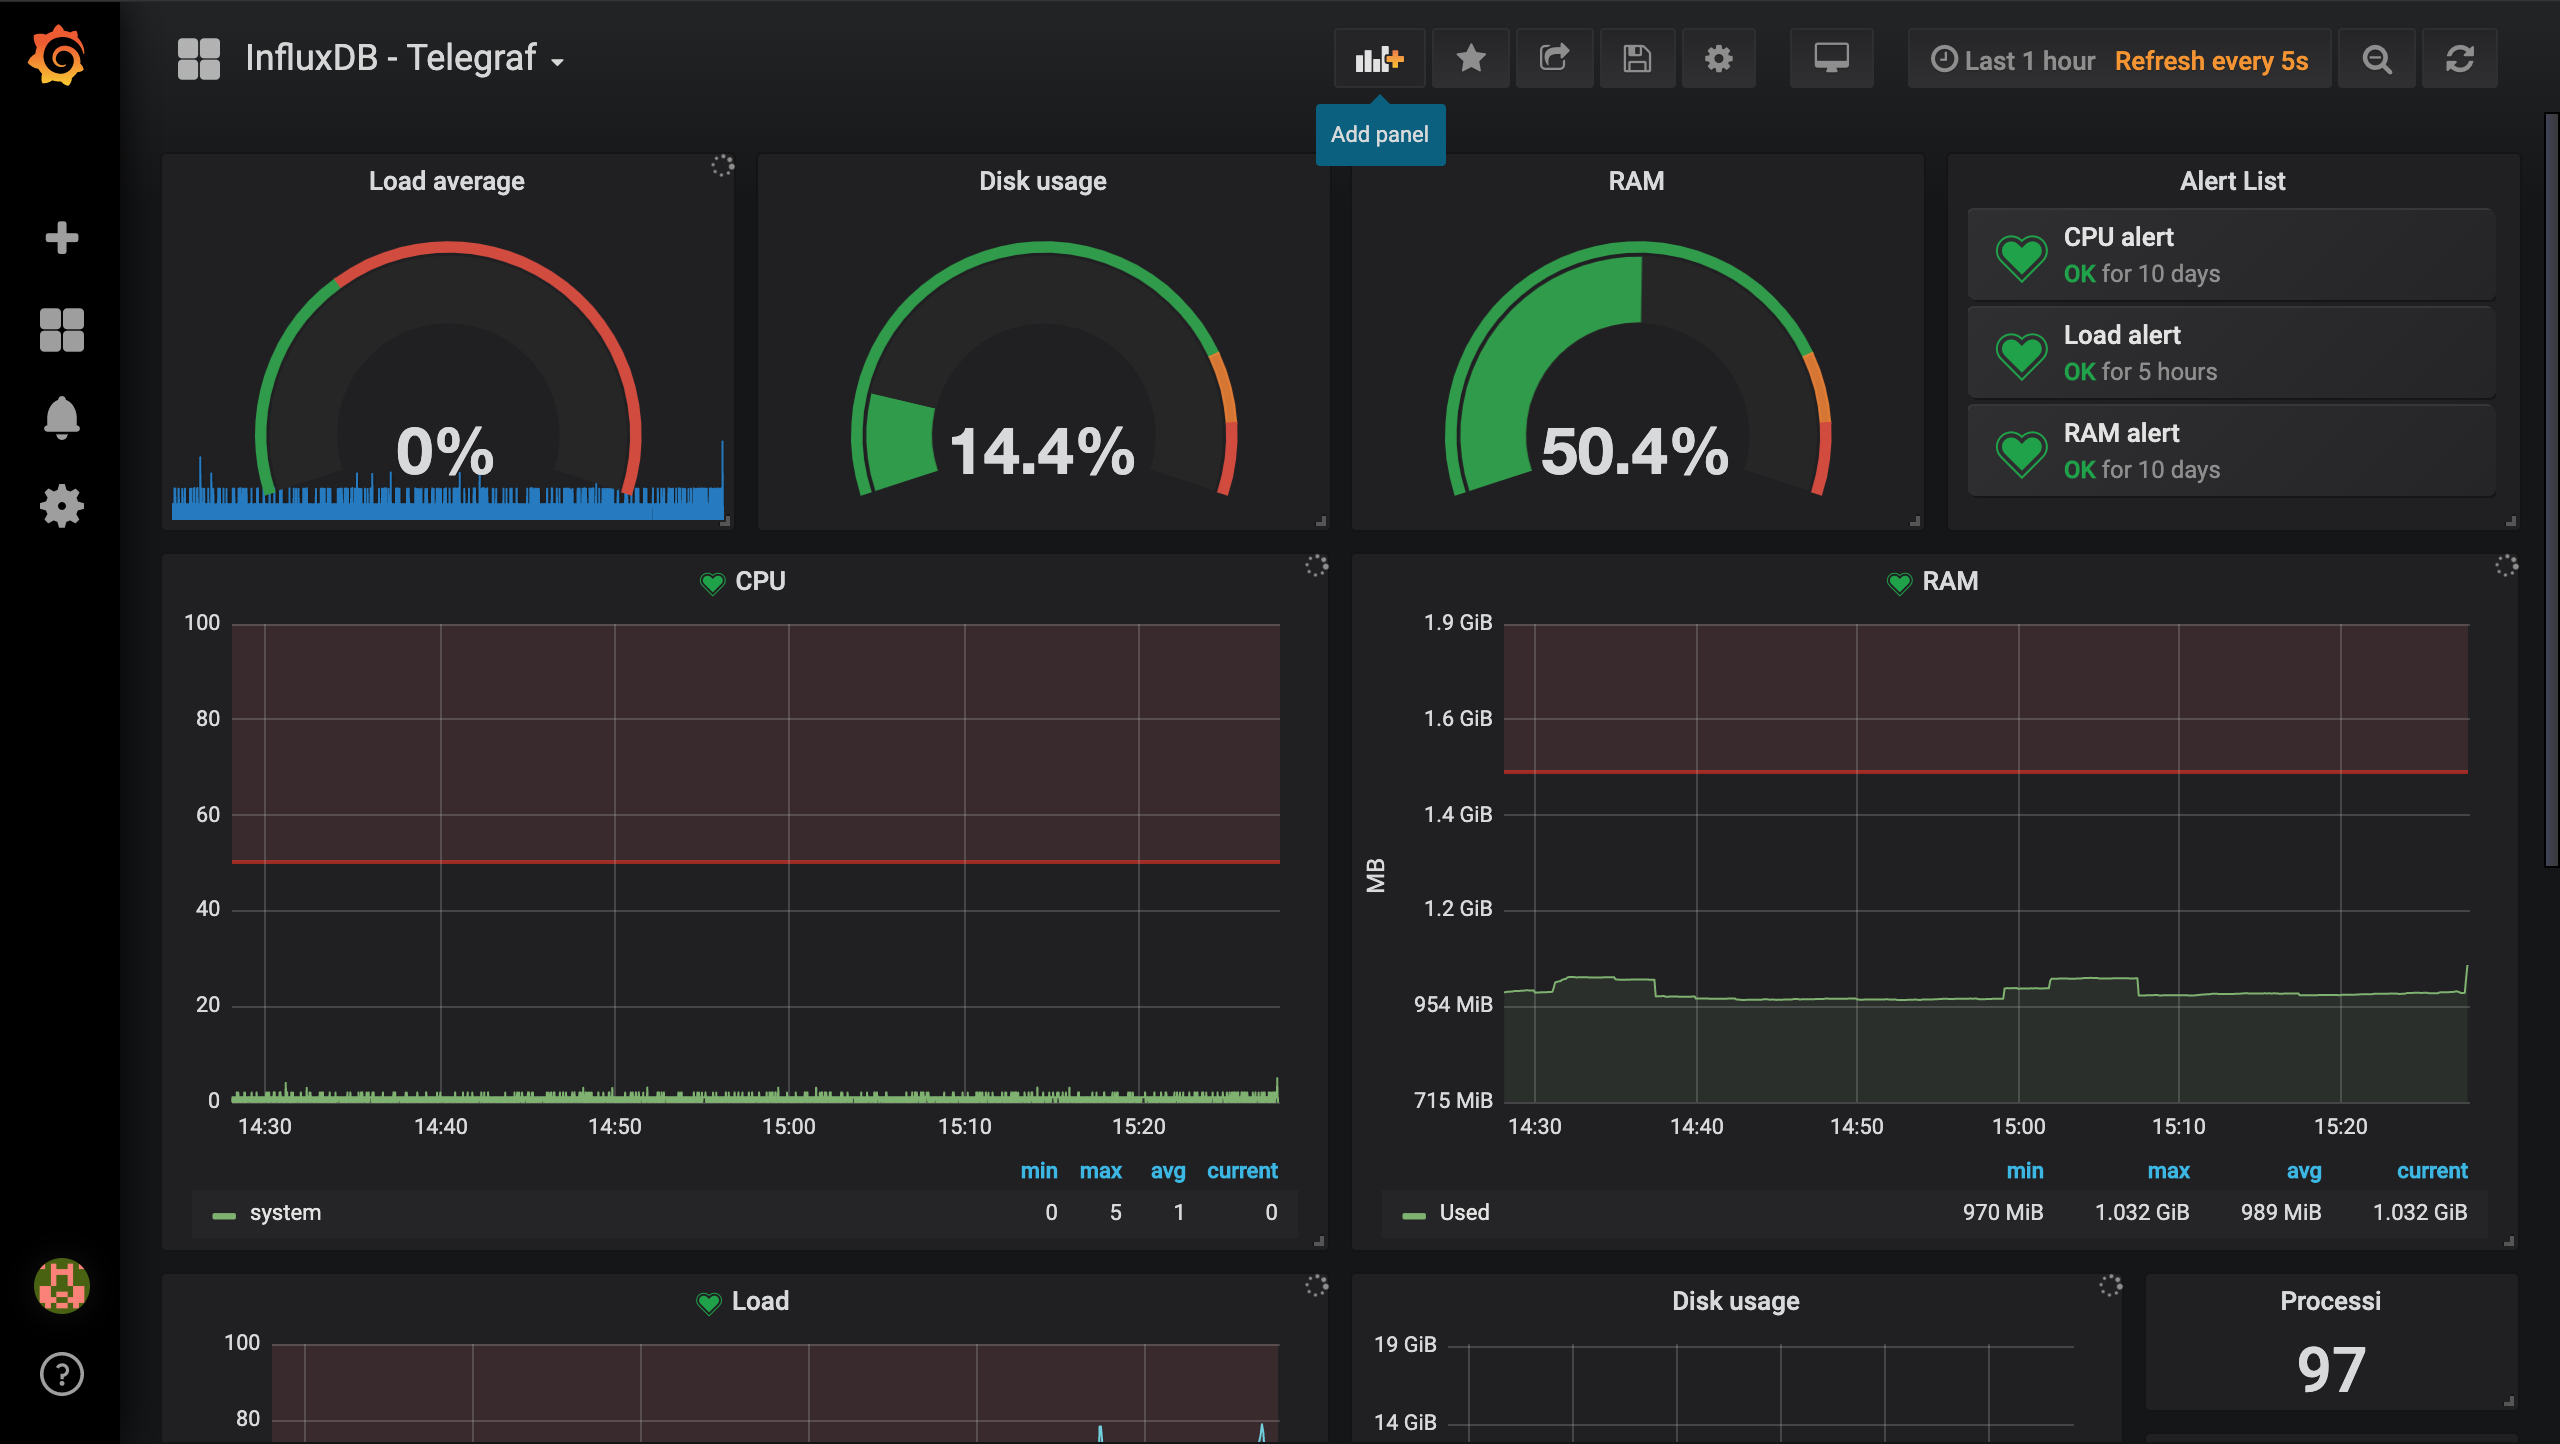
\includegraphics[scale=0.33]{./images/Dashboard.png}
		 \caption{Dashboard di esempio della piattaforma Grafana}	
		 \label{Dashboard}
	\end{center}
\end{figure}

La Figura \ref{Dashboard} espone una Dashboard di esempio, con evidenziato il dettaglio dell'hover causato dal mouse posizionato sul pulsante \textbf{Add panel}.\\
L'operazione di aggiunta del pannello si compone di tre passaggi:
~\\

\textbf{PASSAGGIO 1:} L'utente clicca il pulsante "Add panel" posizionato centralmente nella parte superiore della dashboard. Nella Figura \ref{Dashboard} è visibile l'effetto di hover di tale pulsante.
~\\

\textbf{PASSAGGIO 2:} L'utente visualizza ora il nuovo pannello appena aggiunto (Figura \ref{NewPanel}), e deve quindi definirne la visualizzazione cliccando \textbf{Choose Visualization}.

\begin{figure}[H]
	\begin{center}
		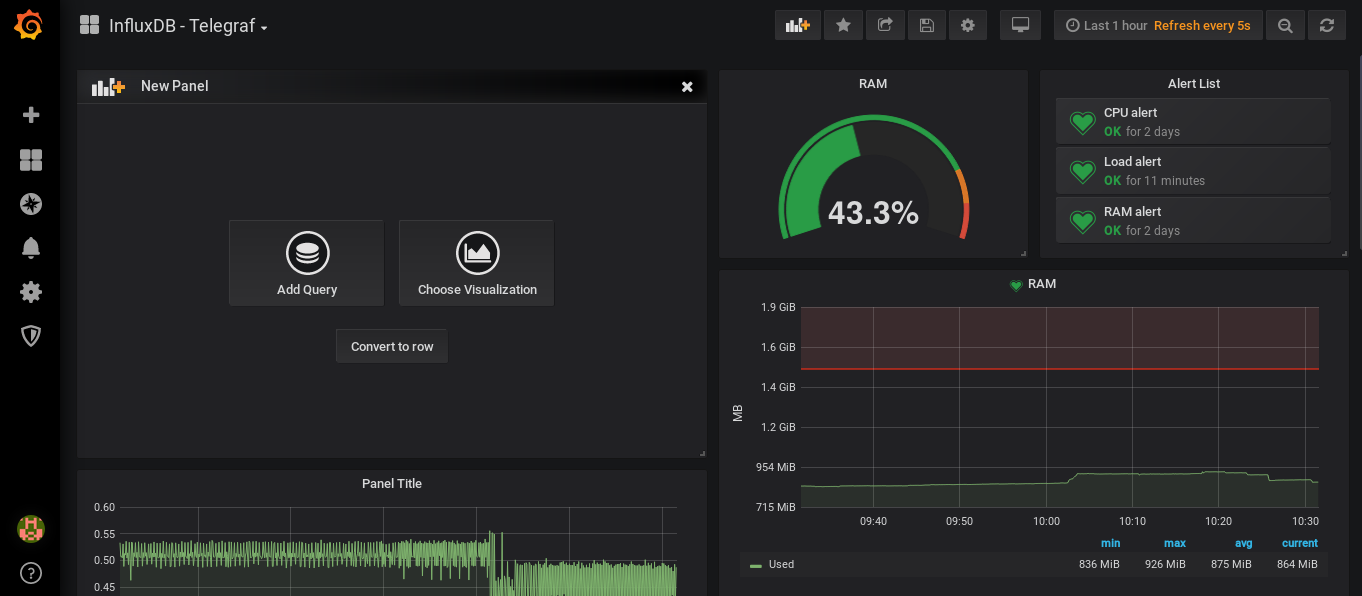
\includegraphics[scale=0.31]{./images/NewPanel.png}
		 \caption{Visualizzazione del "Nuovo Pannello" appena aggiunto alla Dashboard}	
		 \label{NewPanel}
	\end{center}
\end{figure}

\textbf{PASSAGGIO 3:} L'utente deve dunque selezionare la visualizzazione \textbf{Bayesian Networks} per selezionare il pannello \textit{G\&B} (Figura \ref{AddPanelImg}).

\begin{figure}[H]
	\begin{center}
		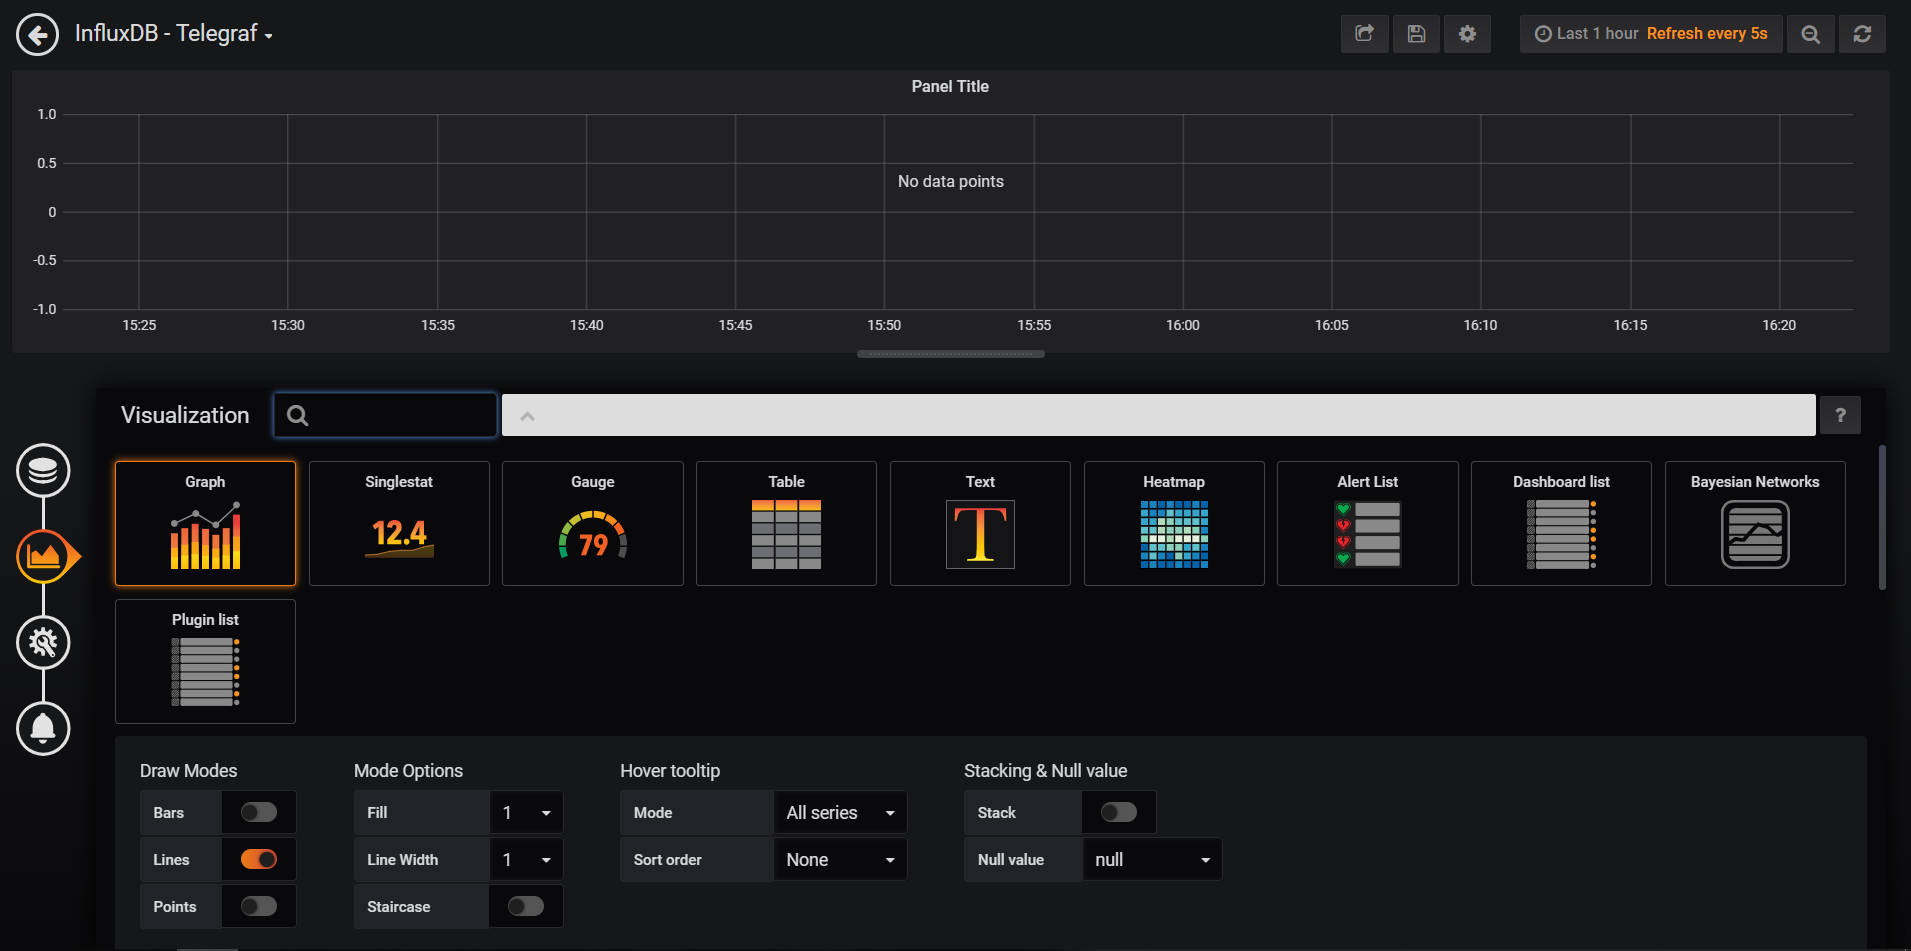
\includegraphics[scale=0.37]{./images/AddPanel.png}
		 \caption{Selezione della visualizzazione del Nuovo Pannello}	
		 \label{AddPanelImg}
	\end{center}
\end{figure}


L'utente può dunque tornare alla visualizzazione della propria Dashboard, ora arricchita dal pannello \textit{G\&B} appena aggiunto (Figura \ref{DashboardPanel}), premendo il pulsante di "Indietro" (visibile in Figura \ref{AddPanelImg}).

\begin{figure}[H]
	\begin{center}
		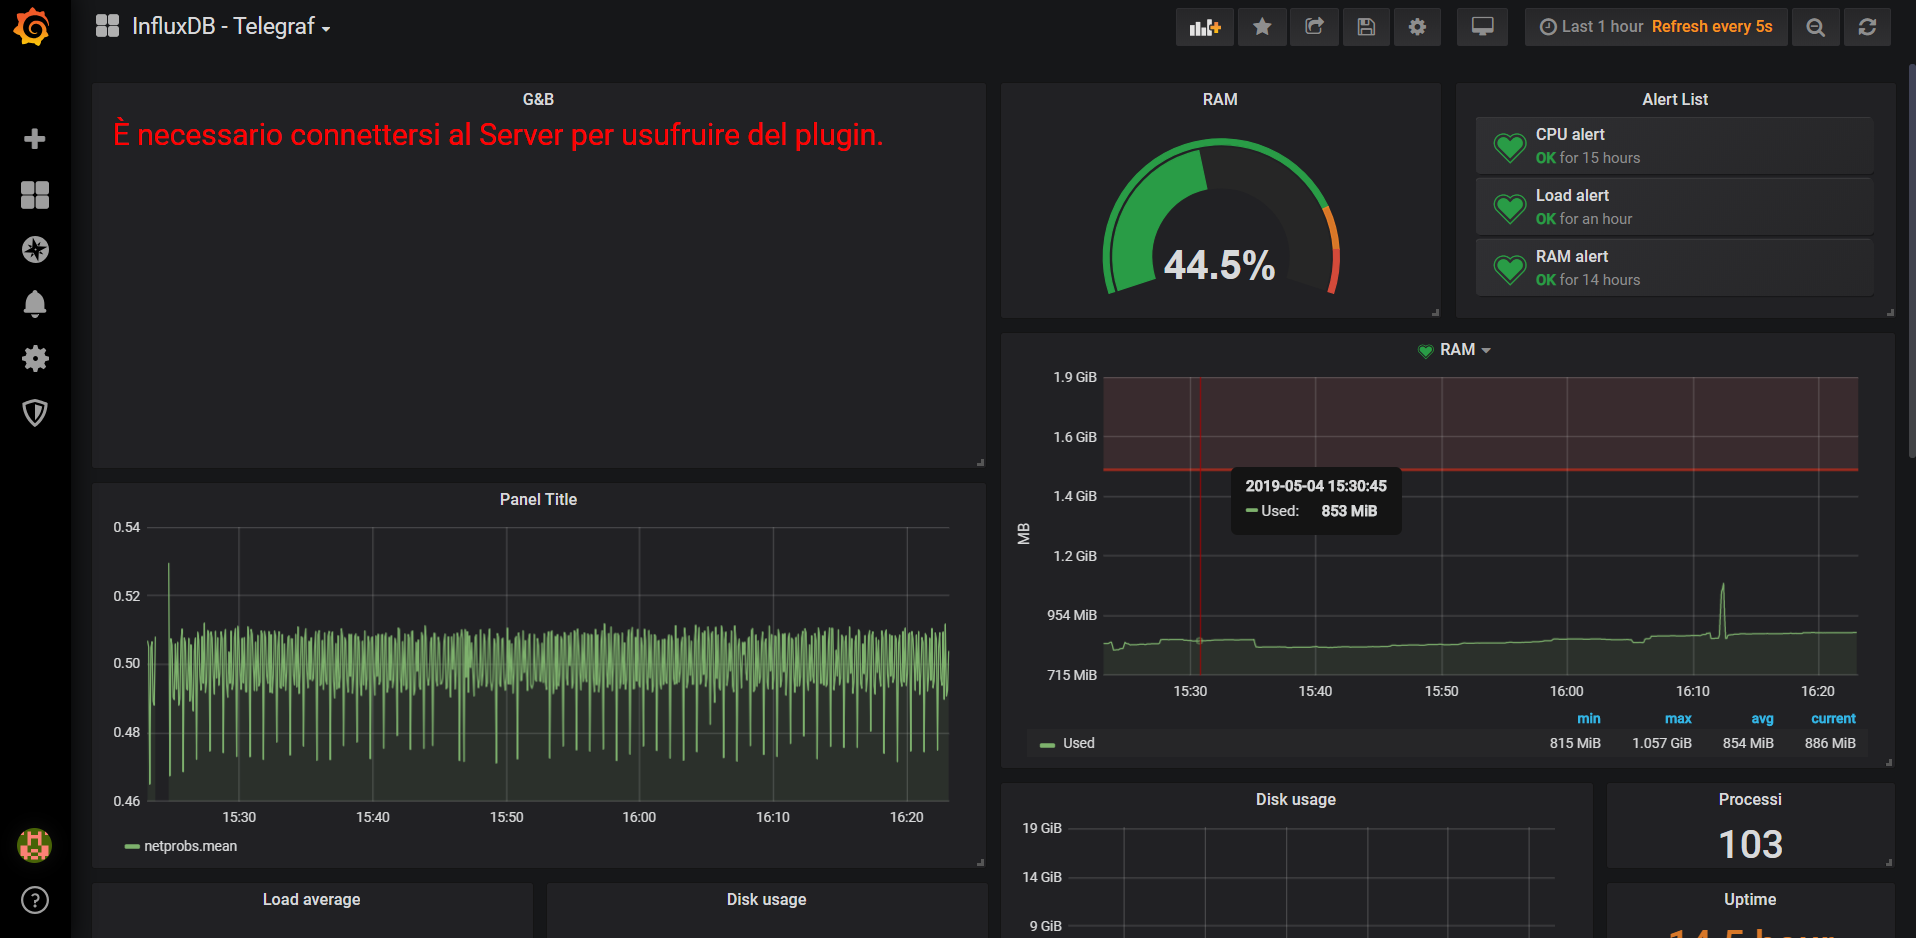
\includegraphics[scale=0.37]{./images/DashboardPanel.png}
		 \caption{Dashboard di Grafana contente il pannello G\&B}	
		 \label{DashboardPanel}
	\end{center}
\end{figure}
